%%%%%%%%%%%%%%%%%%%%%%%%%%%%%%%%%%%%%%%%%%%%%%%%%%%%%%%%%%%%%%%%%%%%%%%%%%%%%%%%
%2345678901234567890123456789012345678901234567890123456789012345678901234567890
%        1         2         3         4         5         6         7         8

\documentclass[letterpaper, 10 pt, conference]{ieeeconf}  % Comment this line out
                                                          % if you need a4paper
%\documentclass[a4paper, 10pt, conference]{ieeeconf}      % Use this line for a4
                                                          % paper

\IEEEoverridecommandlockouts                              % This command is only
                                                          % needed if you want to
                                                          % use the \thanks command
\overrideIEEEmargins
\let\labelindent\relax

% See the \addtolength command later in the file to balance the column lengths
% on the last page of the document



% The following packages can be found on http:\\www.ctan.org
\usepackage{graphics} % for pdf, bitmapped graphics files
%\usepackage{epsfig} % for postscript graphics files
%\usepackage{mathptmx} % assumes new font selection scheme installed
%\usepackage{times} % assumes new font selection scheme installed
%\usepackage{amsmath} % assumes amsmath package installed
%\usepackage{amssymb}  % assumes amsmath package installed
\let\proof\relax
\let\endproof\relax
\usepackage{amsthm}
\theoremstyle{definition}
\newtheorem{definition}{Definition}
\graphicspath{{images/}}
\usepackage{xcolor,soul}
\usepackage[inline, shortlabels]{enumitem}
\usepackage{biblatex}
\renewcommand*{\bibfont}{\small}
% personal productivity
\usepackage[colorinlistoftodos]{todonotes}
\presetkeys{todonotes}{inline}{}
\usepackage{hyperref}
\newcommand{\toread}[1]{\todo[color=red!40!white]{#1}}
\newcommand{\towrite}[1]{\todo[color=blue!40!white]{#1}}
\renewcommand{\hl}[1]{{\color{red}#1}}
\AtEveryBibitem{%
\ifentrytype{book}{
    \clearfield{url}%
    \clearfield{doi}%
    \clearfield{issn}%
    \clearfield{urldate}%
    \clearfield{review}%
    \clearfield{series}%%
}{}
\ifentrytype{collection}{
    \clearfield{url}%
    \clearfield{doi}%
    \clearfield{issn}%
    \clearfield{urldate}%
    \clearfield{review}%
    \clearfield{series}%%
}{}
\ifentrytype{incollection}{
    \clearfield{url}%
    \clearfield{doi}%
    \clearfield{issn}%
    \clearfield{urldate}%
    \clearfield{review}%
    \clearfield{series}%%
}{}
\ifentrytype{article}{
    \clearfield{url}%
    \clearfield{doi}%
    \clearfield{issn}%
    \clearfield{urldate}%
    \clearfield{review}%
    \clearfield{series}%%
}{}
\ifentrytype{inproceedings}{
    \clearfield{url}%
    \clearfield{doi}%
    \clearfield{issn}%
    \clearfield{urldate}%
    \clearfield{review}%
    \clearfield{series}%%
}{}
\ifentrytype{techreport}{
    \clearfield{url}%
    \clearfield{doi}%
    \clearfield{issn}%
    \clearfield{urldate}%
    \clearfield{review}%
    \clearfield{series}%%
}{}
\ifentrytype{misc}{
    \clearfield{url}%
    \clearfield{doi}%
    \clearfield{issn}%
    \clearfield{urldate}%
    \clearfield{review}%
    \clearfield{series}%%
}{}
}

\bibliography{rexam}

\title{\LARGE \bf
A Taxonomy for Characterizing Modes of Interactions in Goal-driven, Human-robot Teams
}
\newcommand{\citet}[1]{\citeauthor{#1}~\cite{#1}}
%\author{ \parbox{3 in}{\centering Huibert Kwakernaak*
%         \thanks{*Use the $\backslash$thanks command to put information here}\\
%         Faculty of Electrical Engineering, Mathematics and Computer Science\\
%         University of Twente\\
%         7500 AE Enschede, The Netherlands\\
%         {\tt\small h.kwakernaak@autsubmit.com}}
%         \hspace*{ 0.5 in}
%         \parbox{3 in}{ \centering Pradeep Misra**
%         \thanks{**The footnote marks may be inserted manually}\\
%        Department of Electrical Engineering \\
%         Wright State University\\
%         Dayton, OH 45435, USA\\
%         {\tt\small pmisra@cs.wright.edu}}
%}

\author{
Priyam Parashar, Lindsay M. Sanneman, Julie A. Shah, Henrik I. Christensen
}


\begin{document}



\maketitle
\thispagestyle{empty}
\pagestyle{empty}


%%%%%%%%%%%%%%%%%%%%%%%%%%%%%%%%%%%%%%%%%%%%%%%%%%%%%%%%%%%%%%%%%%%%%%%%%%%%%%%%
\begin{abstract}

As robots and other autonomous agents are incorporated into increasingly complex domains, classifying interaction in heterogeneous teams including both humans and automation is necessary. Previous literature has addressed the task of classifying human-robot interaction from different aspects and situated in different contexts. However, the factors behind an interaction work in unison and the insights from one perspective inadvertently affect the other. This motivates a need for unification of these taxonomies and framework within an upper ontology which can systematically define these relationships. In this paper we review existing taxonomies from human-robot interaction, the behavioral sciences, social taxonomies, and algorithmic taxonomies and propose an upper ontology over these works. We identify three main components characterizing interaction systems: task, environment, and team, and structure them over two levels: contextual factors and factors driven by local dynamics. Finally, we identify a classification of the effects given contextual factors and local dynamics and discuss open areas of research motivated by the observed gaps in the literature. 

\end{abstract}


%%%%%%%%%%%%%%%%%%%%%%%%%%%%%%%%%%%%%%%%%%%%%%%%%%%%%%%%%%%%%%%%%%%%%%%%%%%%%%%%

\section{INTRODUCTION}
\label{sec:intro}

\subsection{IROS Intro}

Applicability of robotics has extended beyond a single autonomous agent interacting with a single human to scenarios involving larger heterogeneous teams of multiple, functionally-different autonomous agents and humans working together \cite{Burke2004}.
Existing taxonomies characterize individual factors impacting interaction in these increasingly complex domains \cite{Beer2017,cao1997cooperative,Dudek2002updated,Goodrich2007,JiangArkin2015, Korsah2013, Yanco2004updated}, but none comprehensively covers the space. This is demonstrated by a domain in which multiple humans and robots are interacting to jointly accomplish an assembly task. The humans and robots are each assigned a set of tasks and need to collaborate to execute them in the correct order, with the correct timing, and without impeding the progress of each other. Interaction in this scenario is driven by a number of factors including team composition and capabilities, the type of task being executed, whether planning and execution is taking place in a centralized or decentralized fashion, the spatial relationship of the humans and robots, and task and schedule dependencies between different teammates.  
\cite{cao1997cooperative, Dudek2002updated} propose classifications for team composition and capabilities, and \cite{Yanco2004updated} incorporates factors like task criticality and spatial relationships. However, neither of these explore aspects of schedule dependencies between different tasks that teammates are performing as in \cite{Korsah2013}, and vice versa.
\citet{Beer2014toward} propose a framework for estimating the level of robot autonomy for perception, planning and decision stages of a task.
However dynamic scenarios require these to be changed from one sub-task to another which underscores the need for a structured  way of updating the awareness of the agents for the current status of the task and space \cite{chen2018situation, endsley1988design}.

The primary aim of this paper is to propose a unified upper ontology with the dual purpose of preserving the interactions between the surveyed taxonomies while allowing for extending their structures for the characterization of human-autonomous agent interaction in these increasingly complex scenarios. We analyzed existing taxonomies studying interactions in human-robot teams. This body of literature drew from works exploring interaction in the behavioral sciences \cite{chen2018situation, endsley1988design, Mathieu2000TheIO} and social contexts \cite{Fong2003, Goodrich2007} and algorithmic techniques driving interaction in human-robot teams \cite{Korsah2013, Beer2017}. In this work, we propose a framework that will more comprehensively classify factors impacting interaction and highlight areas where this framework can be extended in the future. 

\subsection{Old Intro}

The applicability of robots is extending beyond a single autonomous agent interacting with a single human to scenarios involving larger heterogeneous teams of multiple, functionally-different autonomous agents and humans working together \cite{Burke2004Miami}.
Additionally, interaction between humans and autonomous agents has transformed from simple tasks in human-engineered environments to more complex domains characterized by partially-known and dynamic environments \cite{Casper2003, Burke2004Miami}, novel and unmodeled tasks \cite{fitzgerald2018human, Cakmak2010}, and unstructured human and agent populations within teams \cite{Thrun1999Minerva, Burgard1999Mesuem,pacchierotti2006design}.
These domains require new informational abstractions and representations to support information sharing and collaborative decision-making. 

While there is a wealth of literature exploring one-to-one human-agent interaction in structured domains, as autonomous agents are incorporated into larger heterogeneous teams in unstructured environments, it becomes increasingly important to define how information will be shared between teammates and sub-teams in pursuit of shared goals in these novel domains \cite{Karma2015, chen2018situation, Korsah2013}. To this end, in this paper we characterize needs for information sharing and interaction within heterogeneous teams in complex scenarios by surveying the literature and defining an upper ontology that details important factors impacting interaction in these domains. For our analysis, we analyzed existing taxonomies studying interactions in human-robot teams and literature studying interactions as a means to an end. This body of literature drew from works exploring interaction in the behavioral sciences \cite{chen2018situation, Endsley1995, Mathieu2000TheIO} and social contexts \cite{Fong2003, Goodrich2007} and algorithmic techniques driving interaction in human-robot teams \cite{Korsah2013, Beer2017}. 

We aim to understand how to characterize needs for information sharing and interaction within heterogeneous teams in complex scenarios and to highlight areas for further research.
Specifically, we focus on interactions in a heterogeneous team, where human(s) and robot(s) are involved in a shared activity.
The activity must have a shared task workflow or shared goal.
As a first step, we systematically review taxonomies already proposed over HRI problems and create an upper ontology which highlights the relevant features as seen from different perspectives.
In this paper we additionally integrate the insights from reviewed literature with the idea of individual and team situational awareness as the sum of a priori situational awareness and information acquired through interaction and explore how interaction is necessarily determined at least in part by the informational needs of each role in the team.


\cite{Yanco2004updated} define a taxonomy for human-robot interaction that incorporates aspects of task structure and team composition, including robot features and roles of the human with respect to the robot(s) in the team. Additionally, \cite{Beer2017} explores a framework for multi-human multi-robot interaction that takes into consideration the team, task, and environment structures for a given scenario and the corresponding goals and constraints within the given context. While we see valuable insights in these works and build on the structures they propose, these works and others largely assume static roles for humans and autonomous agents operating in teams. As capabilities of autonomous agents are extended and teams are consequently afforded greater flexibility in pursuit of shared goals, a framework that defines interaction requirements in terms of roles within the team, agnostic as to whether the role is filled by a human or an autonomous agent, is necessary. The primary aim of this paper, therefore, is to propose an upper ontology over existing taxonomies and literature that extends existing structures in a way that allows for definition of human-autonomous agent interaction in these increasingly complex scenarios characterized by greater flexibility.

[cite Yanco] defines a taxonomy for human-robot interaction that incorporates aspects of task structure and team composition, including robot features and roles of the human with respect to the robot(s) in the team. Additionally, [cite Beer] explores a framework for multi-human multi-robot interaction that takes into consideration the team, task, and environment structures for a given scenario and the corresponding goals and constraints within the given context. While we see valuable insights in these works and build on the structures they propose, these works and others largely assume static roles for humans and autonomous agents operating in teams. As capabilities of autonomous agents are extended and teams are consequently afforded greater flexibility in pursuit of shared goals, a framework that defines interaction requirements in terms of roles within the team, agnostic as to whether the role is filled by a human or an autonomous agent, is necessary. 

As discussed in [cite Beer], interaction requirements within heterogeneous teams are driven by task, team, and environment structure and composition. We note that environment and task structure in particular drive both physical and cognitive requirements of team members executing tasks and sub-tasks towards a shared goal. While physical requirements for a given task are somewhat more straightforward to define, cognitive requirements involve not only reasoning and decision-making capabilities but also the required situational awareness to support these cognitive processes [add citations here]. Also integral to group success is the support of both individual and group situational awareness which involves information sharing at different levels of abstraction for teammates who are executing different roles within the team and who bring different levels of a priori knowledge to the execution of their assigned tasks. Accordingly, the need for team situational awareness and the existing information gaps within a team drive interaction between teammates or subteams in the form of two-way communication at different levels of abstraction.  Therefore, in this paper we additionally integrate the idea of individual and team situational awareness as the sum of a priori situational awareness and information acquired through interaction and explore how interaction is necessarily determined at least in part by the informational needs of each role in the team. The primary aim of this paper, therefore, is to propose an upper ontology defining human-autonomous agent interaction in heterogeneous teams operating in complex environments. 

 Further, within heterogeneous teams it is important to consider not only the support of individual situational awareness, but also the group situational awareness and shared mental models necessary to support achievement of a shared goal within the team. INSERT OUTLINE.

 

% \begin{figure}[h]
%     \centering
%     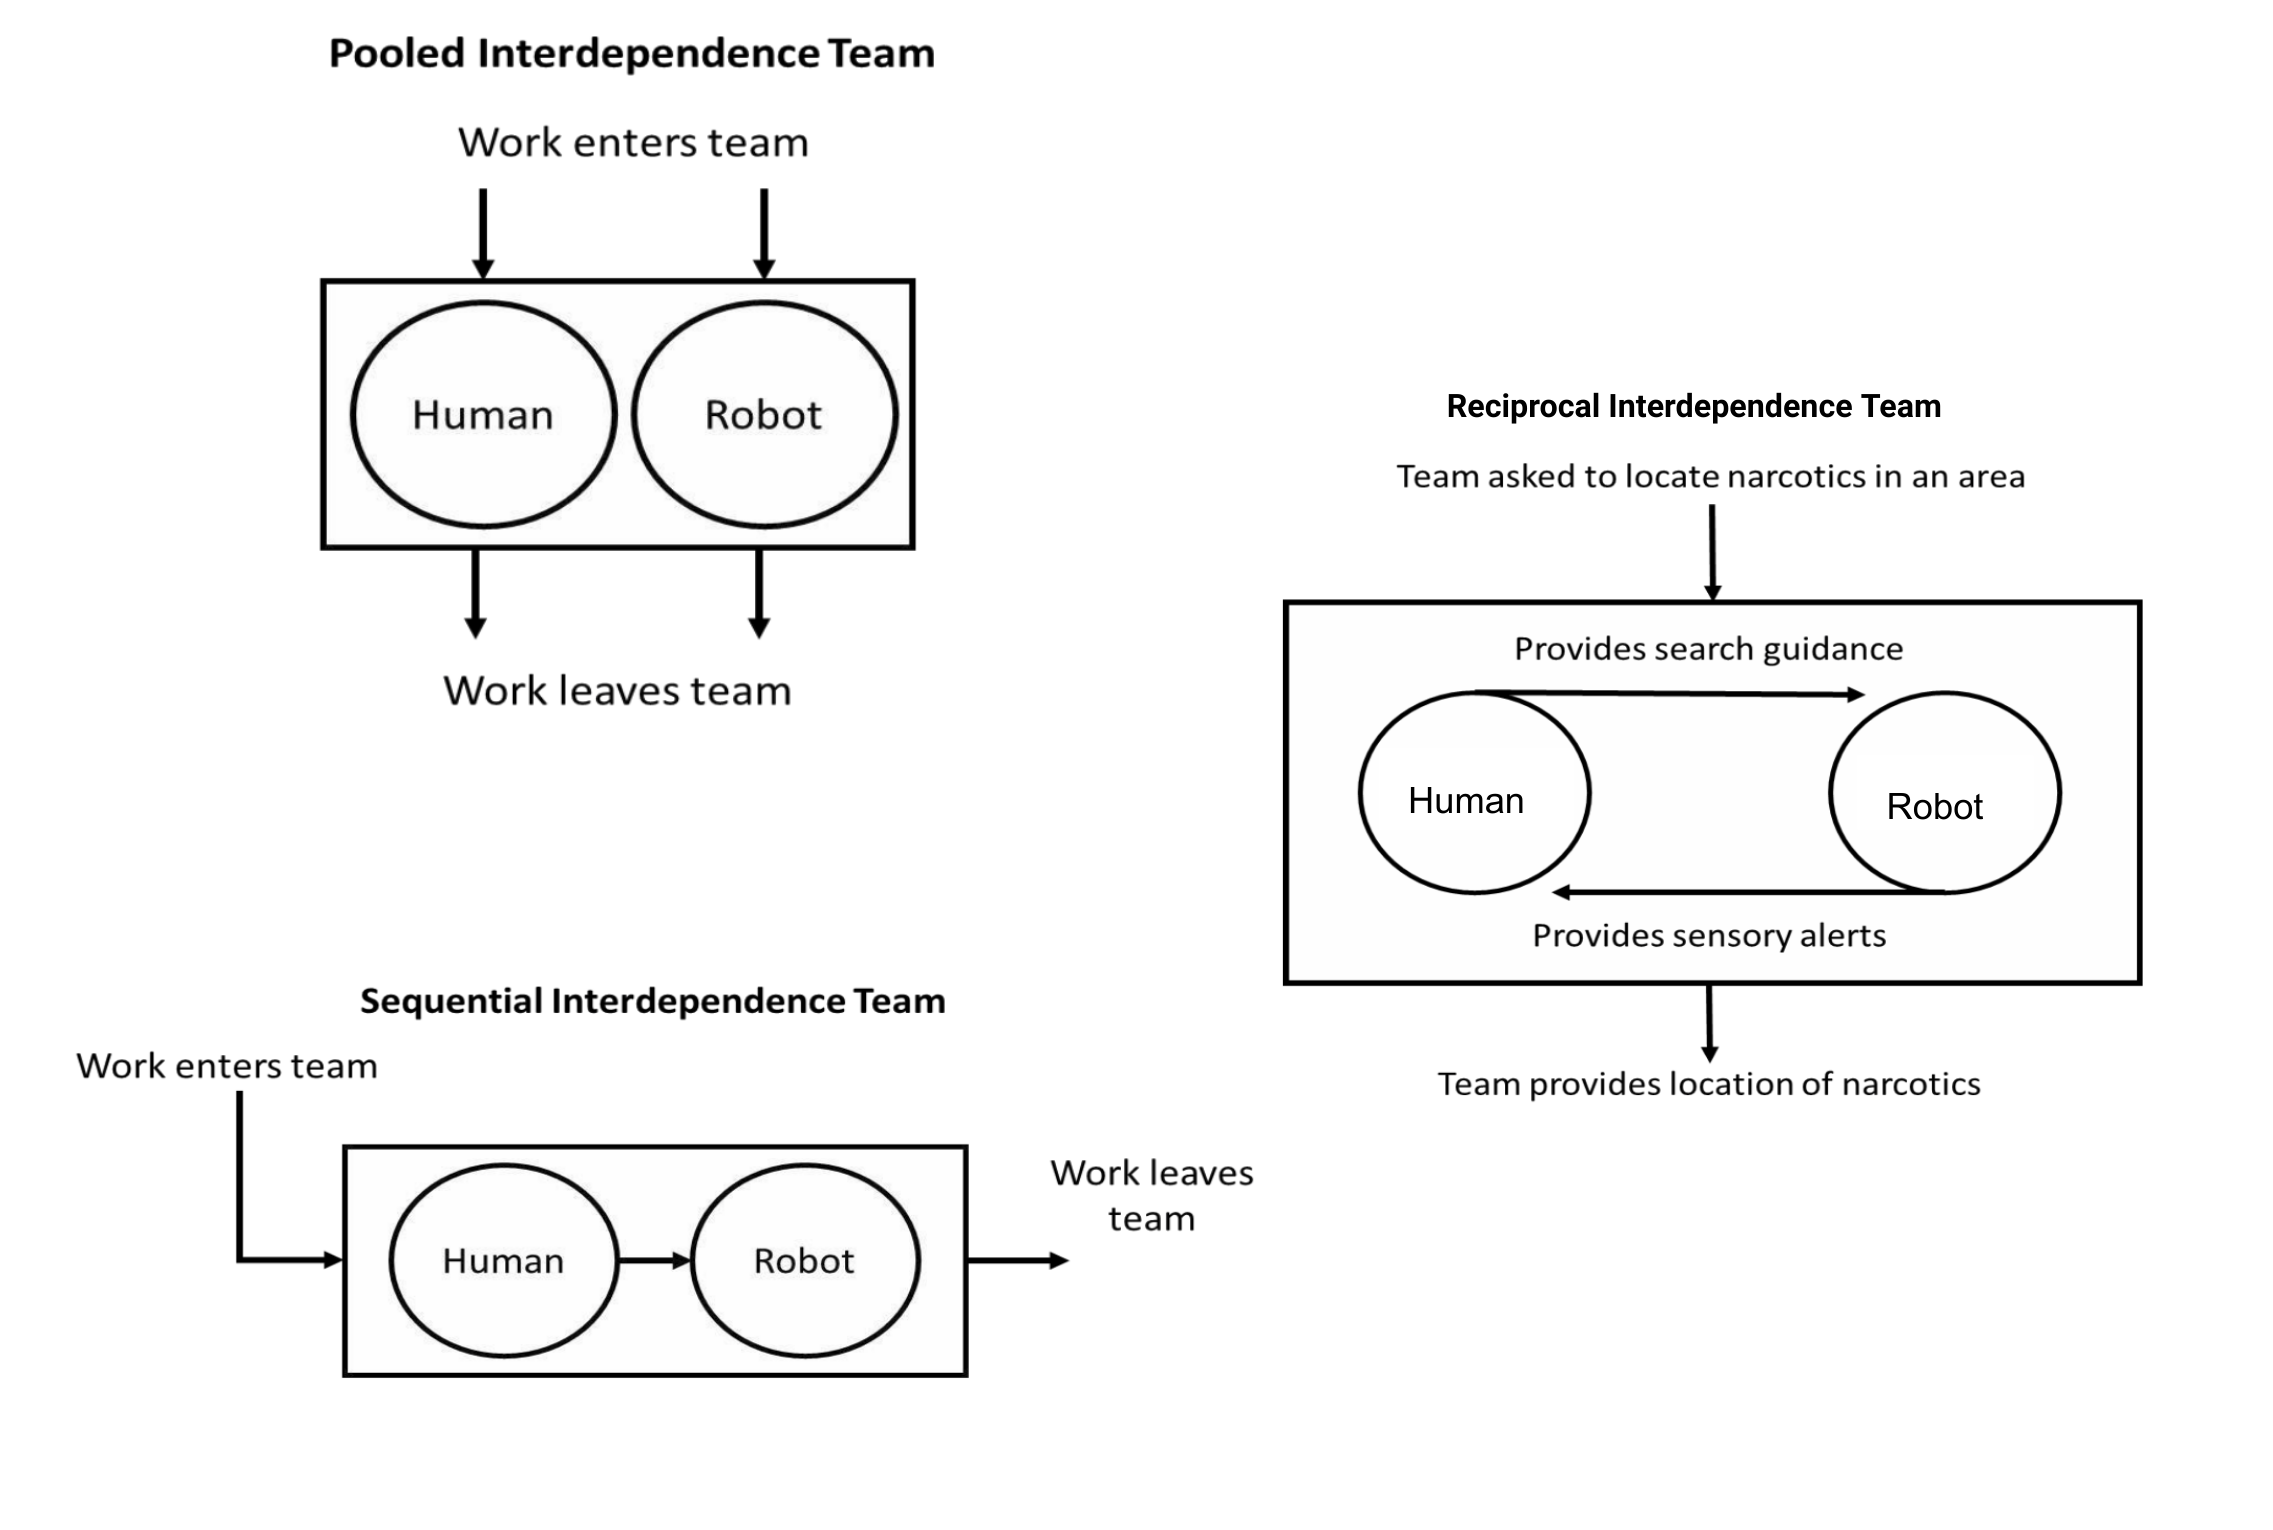
\includegraphics[width=\columnwidth]{task-deps.png}
%     \caption{Visual descriptions of task interdependence scale from \cite{Phillips2015}. Images copied from \cite{Phillips2015} and edited for uniformity.}
%     \label{fig:task-deps}
% \end{figure}

\section{Operational Contexts for Collaborative HRI with Mobile Robots}
\label{sec:op-context}

%\citet{Burke2004} serve as a valuable source of listing applications and domains deemed important by the HRI community.
\citet{Burke2004} present a list of applications and domains deemed relevant to the HRI community.
We reviewed four of the listed operational contexts and observed four macro-themes that introduce complexity in these contexts and are persistent through all four:
\begin{enumerate*}
    \item \textit{environmental} complexity,
    \item knowledge of task goals and priorities or the \textit{task model},
    \item differing nature of other agents or the \textit{team model}, and
    \item level of \textit{risk} to humans and autonomous agents.
\end{enumerate*}
The following scenarios are chosen to illustrate the variety of challenges along the above dimensions. 

\subsection{Interactive Learners (IL )and Museum Docents (MD).}
\label{subsec:il-and-md}
        We outline two predominantly social scenarios where one interactant assumes the expert role and supervises the other towards interacting with the environment, which in turn enhances their knowledge about the task being executed. This is an example of scenarios with a \textit{structured environment}, and the complexity arises from the problem of how to communicate with other agents to enhance their knowledge of underlying \textit{task model} and how to adapt this information to different types of \textit{team models}.
        The interactive learner scenario is a case in which a human acts as a task expert and influences the robot's interactions with the environment to help it learn an optimal cost function representing the goals and constraints of the given task \cite{fitzgerald2018human}.
        In this space, algorithms are developed for robot-novice users such that they can train robots via natural means. Therefore, this requires the robot to be able to support natural language and non-verbal gestures \cite{kidd2006sociable}.
        In the museum docent scenario, a domain-expert robot guides and informs museum-goers such that they can experience the space with a deeper understanding of artifacts exhibited \cite{Thrun1999Minerva, Burgard1999Mesuem, Burke2004}. 
        This also requires support for natural means of communication and is made even more challenging since the human audience is not only robot-novice, but also \textit{multiple} in count.
        
\subsection{Urban search and rescue (USAR).}
\label{subsec:usar}
        This is similar to a typical search and rescue scenario, but instead of using specialized dogs or difficult-to-maneuver tube cameras for the operation, a human remotely operates a robot through physically challenging spaces to search for trapped humans in need of rescue \cite{Casper2003}.
        The robot here is used as an easily-controllable, physically-compact extension of human operator's cognitive, physical, and sensing capabilities.
        This context is complex in terms of \textit{environment} as the areas being scouted are largely \textit{unknown},  \textit{unstructured}, potentially dimly lit which makes perception hard, and \textit{dynamic} since debris can move anytime.
        The risk is high as the environmental factors can pose a danger to both the human operators and the robots in the team \cite{Burke2004Miami, Karma2015}.
        Additionally, since robotic and human teammates might not regularly work together, a gap might also exist between perceived and actual \textit{task} priorities \cite{Casper2003}.
        
        %since most of the robotic teams are not a pre-existing part of the disaster management sub-group, there is also a gap between perceived and actual \textit{task} priorities \cite{Casper2003}.
        
\subsection{Military Building Breach Operation.}
\label{subsec:mbb}
        The military building breach domain is drawn from conversations with domain experts at the Army Research Lab (ARL). It demonstrates complexity in all dimensions, environment, task, and team. Such an operation involves a heterogeneous team of human soldiers, unmanned aerial vehicles, unmanned ground vehicles, and autonomous computer aids working together to navigate an urban environment and breach a building. The task is complex and multi-stage, requiring different abilities and resources for different stages. The planning stage requires team to plan for safely scouting the area and accessing the building while avoiding enemy forces, a scouting stage in which the team checks if the area is clear of enemy forces, a troop movement stage in which the team approaches the building, and finally the building breach. The environment is largely unmapped and dynamic since enemy forces might be encountered, and the team hierarchy is fluid, allowing for changing of roles depending upon arising contingencies and varying abilities of the teammates.
        
        %Similar to the USAR context, the military building breach context entails unmapped, unstructured, and dynamic environmental factors. In this domain, the complexity additionally increases as the team is required to navigate a multi-stage task and there exists an added potential for agents to encounter other \textit{unmodeled adversarial agents}. The building breach scenario involves a mixed team of human soldiers and a heterogeneous set of autonomous agents and autonomous computer aids working together to navigate an urban environment and breach a building. Such missions require physical assistance as well as cognitive support throughout the varying stages of the task.
        %This further adds to the problem of formulating specific informational abstractions which can function independently of the differing abilities of the team-members.
        %The multi-stage task requires different abilities and resources like, planning stage requiring plan for safe scouting, building access and enemy avoidance, scouting stage specifically focusing on monitoring of adversarial troops followed by troop movement stage and finally the building breach.
        %Moreover, the team hierarchy is fluid, allowing for changing of roles depending upon arising contingencies and abilities of the teammates, and the overall risk is high.
% Figure \ref{fig:op-dims} summarizes these dimensions and places the over-viewed contexts within that hyperspace.
% \todo{change op-context-dims figure}
% \begin{figure}[h]
%     \centering
%     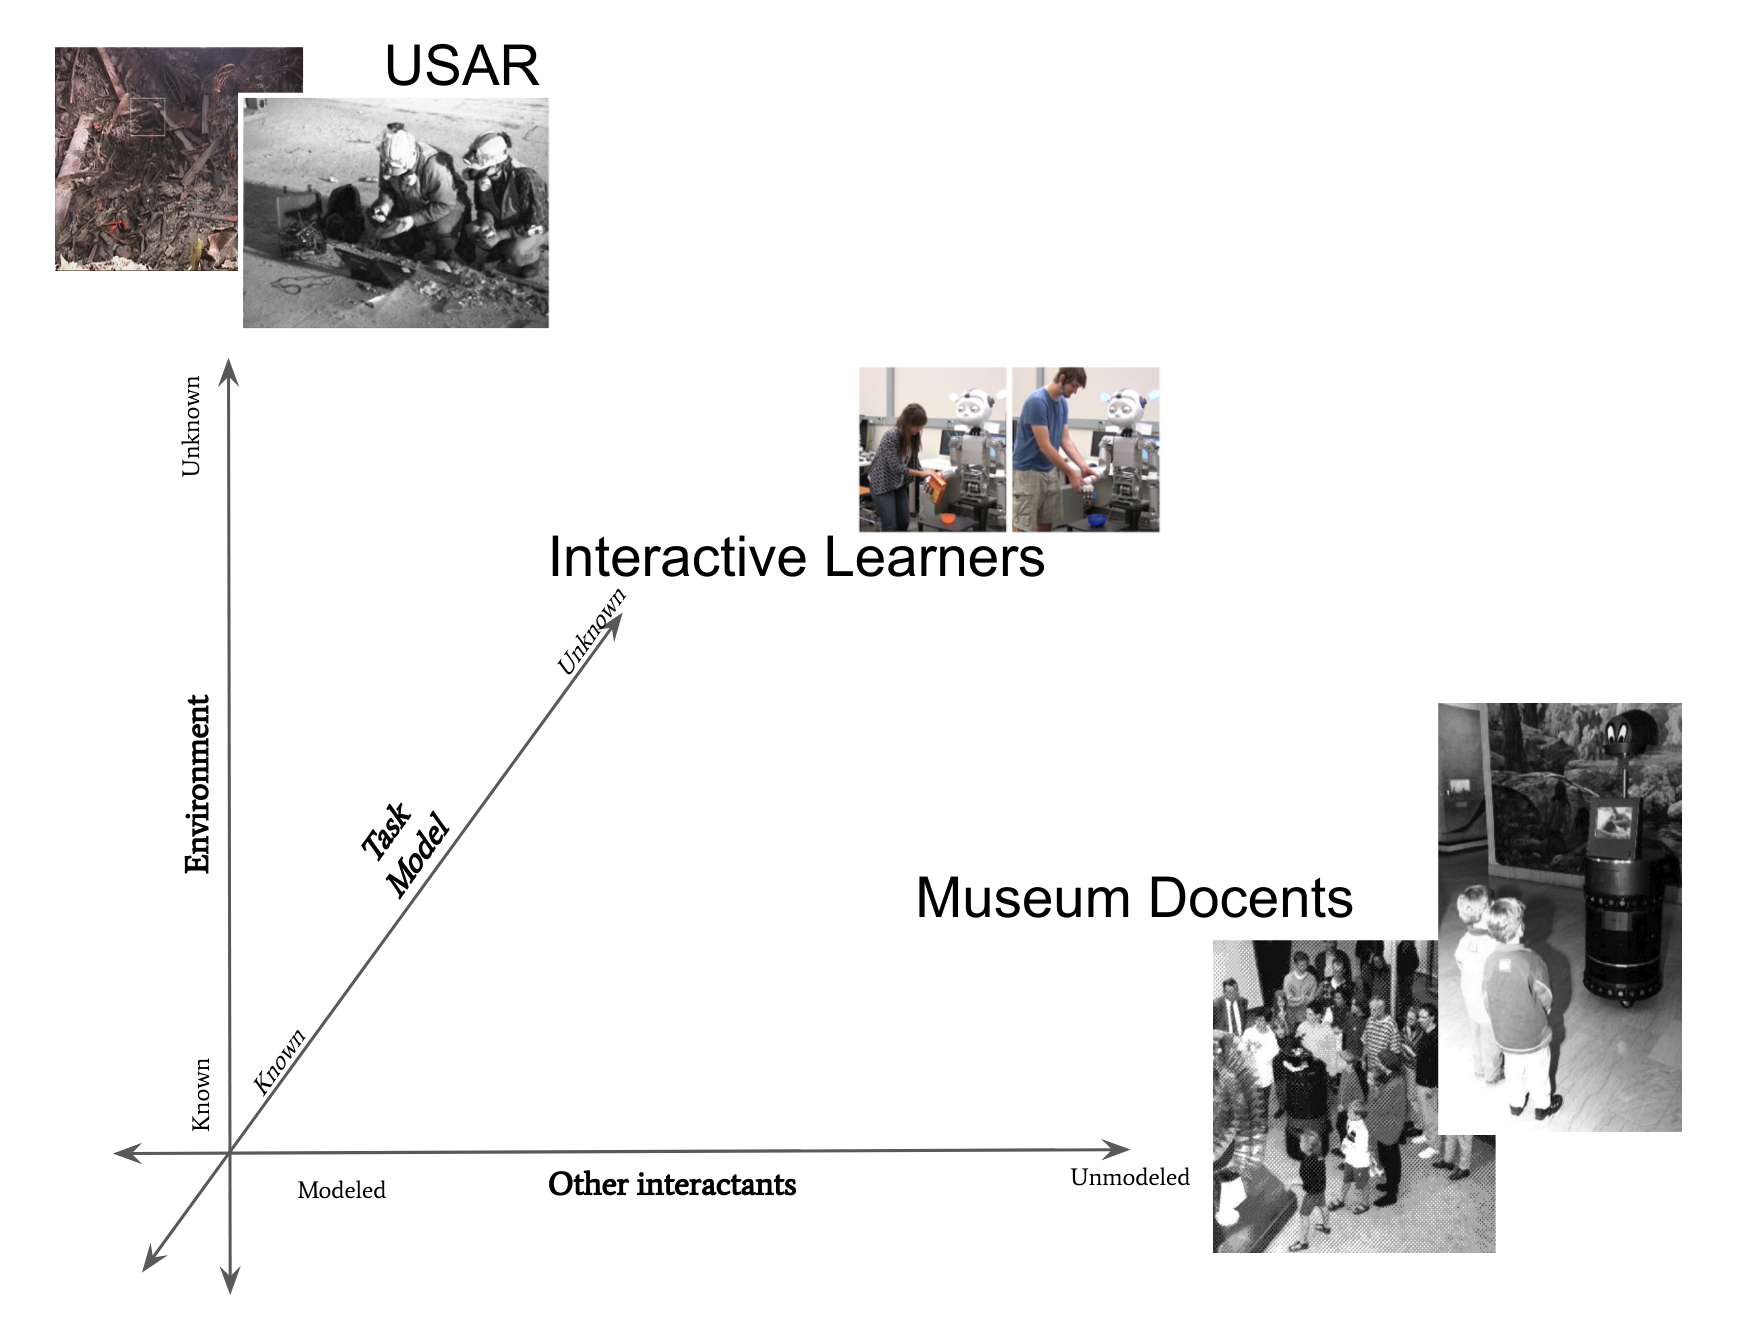
\includegraphics[width=0.5\columnwidth]{op-dims.png}
%     \caption{Major dimensions separating the operational contexts \cite{Casper2003,Cakmak2012, Burgard1999Mesuem, Nourbakhsh1999}}
%     \label{fig:op-dims}
% \end{figure}

\section{An Overview of Existent Taxonomies in HRI}
\label{sec:overview}

Apart from identifying specific dimensions and their effect on interactions, we also found overarching themes over the surveyed taxonomies which influence the structure of the upper ontology proposed in this paper.
For instance, all the taxonomies are designed to address different parts of a cooperative system.
Not only does this differ over lateral components like task context \cite{Beer2017} and team configuration \cite{Dudek2002updated, cao1997cooperative}, but also over different levels of depth, i.e. from macro-\textit{context} \cite{Yanco2004updated} to local complexities or \textit{dynamics} of a specific task instantiation \cite{Korsah2013, Beer2014toward}.
Furthermore since each taxonomy describes interactions within a smaller context, we did not find an explicit characterization of \textit{environment} context which we identified as instrumental to characterizing the challenges to the system in \ref{subsec:usar} anf \ref{subsec:mbb}.
Additionally, we observed multiple taxonomies presenting a discussion over similar topics like \textit{task interdependency} and \textit{level of robot autonomy} under different names or from different investigational perspectives.
In our new taxonomy we include the insights from these taxonomies to break-down these concepts further along these varying dimensions.
We present the surveyed taxonomies categorized under a similar structure as they have informed for our formulated taxonomy.\footnote{Note that some taxonomies present variables for local dynamics along-side contextual variables so the discussion is divided for over two different sections.}

\subsection{Context-driven Taxonomies}
We briefly define contextual taxonomies as those describing the ``problem'' context and ``solution'' context of an HRI application.
Here the kind of task being undertaken and the complexity of operational environment forms the problem part, while the configuration of the team deployed is identified as the solution.

\subsubsection{Task and Environment as the Problem}
\citeauthor{Yanco2004updated} \cite{Yanco2004updated} provide a meta-survey identifying important factors which are critical to our definition of interaction context.
However, the paper itself does not impose any structure over these dimensions even though they significantly differ in their level of assessment of a system, e.g. while task type is a context-sensitive variable, centralized versus decentralized mode of command consensus is local to the particular role the interactants play in a team hierarchy.
Furthermore, many of the variables specific to local dynamics are affected by the context-level variables, so apart from identifying the important factors it is equally important to elucidate the relationships between them.
More recently \cite{Beer2017} have conducted a work addressing the problem of classifying mixed-team HRI task contexts and the effects on inter-team interactions, but specific to military and commercial operations.
Our upper ontology is influenced by their highest-level of distinction which explains context along the dimensions of: \textit{task focus}, \textit{constraints} and \textit{team configurations}.
Note that while there is an explicit division between task and team-model, environment is relegated to the second-level of categorization used for producing constraints due to the narrow scope of relevant operational contexts.
Apart from enlisting environment as a constraint they also mention that the kind of mission can impose specific constraints on the objective as well, e.g. need for stealth, or speed.
However since there is not a structured framework guiding specific kinds of constraints this serves as more of a guideline than a taxonomic differentiation.
More importantly, \cite{Beer2017} identifies six main task focuses of missions undertaken in military and commercial HRI problems, which we have extended and incorporated in our own upper ontology in section \ref{sec:upper-ontology}.

From the social robotics perspective, \citet{Dautenhahn2007} steps back and asks the question of how can we evaluate criticality of robots to different domains such that social skill development in HRI is justified.
They use four major axes for evaluating HRI application areas: contact with humans, robot functionalities, role of robot and requirements of social skills.
We have included two of those as important dimensions in our taxonomy as a way of typifying the contextual challenges that mixed teams should expect from different operational environments.
\cite{Phillips2015} taking inspiration from human-animal cooperation characterize the type of activity as: \textit{physical} , emotional or more generally \textit{social}, and \textit{cognitive}.
This axis directly maps with the kinds of interactions occurring in outlined contexts of building breach, museum docents and USAR respectively.

\subsubsection{Collective or Solution Specification}

A \textit{collective} here means a heterogeneous team of humans and robots, where the team hierarchy could be flat or not, and the robotic agents can also be heterogeneous in capabilities.
The team context specifies macro-dimensions like the size and composition of the group \cite{Beer2017}, and communication constraints imposed by system design \cite{Dudek2002updated, cao1997cooperative}.
Another important aspect is the a priori modeling of teammates to better understand their needs during execution.
\cite{cao1997cooperative} employ a belief-desire-intention model to describe agents, while \cite{stone2000multiagent} define heterogeneous agents by their goals, actions and knowledge structures.
% Table\hl{reference to table} lists the specific dimensions borrowed from the surveyed papers for typifying team configuration.

\subsection{Cooperation-driven Taxonomies}

In an attempt to understand natural cooperation better, the HRI community has studied human-animal interactions to develop guidelines and descriptive categorizations for future human-robot team-tasks.
\cite{Phillips2015} identify the frequency of communication and task-flow interdependency between two interactants as critical to characterizing the level of cooperation between them.
They break task-interdependence into three modes which specify parallel, sequential and dialog-like modes of working on a task.
This dimension of interdependence is echoed in \cite{GerkeyMataric2004, Korsah2013} from the perspective of task allocation.
They divide task interdependence over two major dimensions of inter-agent task labor division and the scheduling constraints between the allocated sub-tasks.
This categorization presents a more systematic breakdown than \cite{Phillips2015} and is included in our taxonomy.
In similar vein, \cite{Beer2014toward, JiangArkin2015} illustrate a strong link between the projected criticality of a task, in terms of life-risk and importance to mission success, and the chosen levels of robot autonomy for a mixed system.
Both \cite{Beer2014toward, JiangArkin2015} define level of robot autonomy as a spectrum of responsibility or initiative overlap over the different task-stages and goal milestones, respectively.
\cite{Beer2014toward} outlines 10 specific configurations of these possible responsibility overlaps during task execution by deconstructing the task as a sense-plan-act cycle \cite{murphy2000introduction}.

One of the most important behavioral factors shaping human-robot interaction, which we have implicitly mentioned before, is the role of the human.
Scholtz \cite{Scholtz2003} used Norman's seven-stage model of interaction design \cite{Norman1986} to reflect on the failure of robots and typify related assistance required by the intermediate layers of intention, action and perception in the agent.
This led to formulation of the 5 archetypal roles humans can play to help the robot.
Interestingly, Norman used his model for conceptualizing human-centric designs, however \cite{Scholtz2003} flips the model to come up with a robot-centric view of usefulness of human knowledge such that the combined human-robot system is usable.
It warrants mention that since robotic technology is increasingly ubiquitous in the human-occupied world, there is a space for conception of additional collaborative human-robot roles.
This role-call was last updated in 2007 \cite{Goodrich2007} with the addition of two new entries(*), one of which is specifically robot-centric (emphasized): \begin{enumerate*}
    \item supervisor,
    \item operator,
    \item mechanic,
    \item peer,
    \item bystander,
    \item *\textit{mentor}, and
    \item *information consumer.
\end{enumerate*}
The papers do a good job of explaining ``why'' such roles are needed to make a system usable and presents a detailed synopsis of ``what'' information the system designers should focus on while designing a human-robot interface for these roles.
However, as we move towards a more cooperative landscape of HRI we will need the autonomous agents to fluidly move through a team hierarchy and wear different hats during different contexts, just as we expect from a collaborative team of humans.
This entails that the expectations of expertise and knowledge from these roles need to be quantified by grounding it within the mission context of a mixed team's knowledge structures, enabling an autonomous agent to better validate and support their move from one kind of role to the other.

With a critical eye towards contexts where social interactions are inter-woven with functionality of a team, as compared to being used as a means to another end, \cite{Fong2003, Feil-Seifer, Dautenhahn2007} present a taxonomy identifying the basic components of a robotic system which affect human-robot social interactions.
Focusing on these dimensions from our more generic lens, we found that there is a need for inclusion of training phase of interactions \cite{Fong2003} in the task taxonomies of the past, and we merge this additional aspect with the \textit{task focus} list in \cite{Beer2017} for our taxonomy.
Furthermore, there is additional support to be found for explicitly modeling types of users and the need for a deeper discussion on types of role the human and robot can take in a context where the team hierarchy is more \textit{fluid} \cite{Feil-Seifer, Dautenhahn2007}.

\subsubsection{Information requirements for cooperation}

To study information exchange in interactions we must analyze the question of \textit{what} is the role of this information and \textit{why} must it be disseminated at all?
\citeauthor{endsley1988design} \cite{endsley1988design} provides a framework defining the concept of ``situational awareness'' grounded in the processing mechanisms, design and knowledge of a dynamic system.
It is recognized for the delineation of information into three progressively complex levels of situational awareness (SA).
\citeauthor{chen2018situation} \cite{chen2018situation} ground this model into mission description of a multi-agent interactive task and incorporate information at different levels of plan abstraction for elevated transparency between a robotic agent and the operator.
The following describes this Situation Awareness-Based Agent Transparency (SAT) model with the italicized phrasing describing the level of SA as defined by Endsley.
\begin{itemize}
    \item \textbf{Level 1.} \textit{Perception.} - Current goal, short-term plan, agent status and state.
    \item \textbf{Level 2.} \textit{Comprehension.}\footnote{\cite{Burke2004Miami} adds that comprehension can be of two kinds namely: identification of elements, and interpretation of events under the current situation.} -  Reasoning aspects like belief and purpose in terms of the plan, environment and other constraints.
    \item \textbf{Level 3.} \textit{Projection.} - Projection of finish-time, cost, and uncertainties over future states and goal status.
\end{itemize}

% While classifying modalities is not within the scope of current paper, we want to highlight that for successful interaction the right type of information needs to be supported by the right way of exchanging information.
% \cite{Goodrich2007, Cha2018} provide detailed surveys of modes of communications used in HRI.

\section{Gap Analysis}
\label{sec:analysis}

Our last section identified the need for better understanding of the following aspects of characterization going forward:
\begin{itemize}
    \item A better structure which can encompass the \textit{macro-context} as well as the \textit{local dynamics} while preserving the differentiation between them.
    \item A combined synthesis of dimensions like \textit{task interdependence} and \textit{LORA} which includes the differing perspectives of the surveyed taxonomies.
    \item A need for quantifiable reformulation of roles grounded within the shared knowledge structures of a collective such that they can be used an online framework to assess and validate the informational requirements at different levels.
\end{itemize}

We address the first two issues by proposing a reformulated upper ontology over the surveyed taxonomies in the next section.
Specifically, we include context-driven dimensions from last section to the major category of context further sub-divided into three major classes of: task, team and environment.
These three classes are the result of our analysis of varying operational contexts (section \ref{sec:op-context}) and identified dimensions from \cite{Yanco2004updated, Beer2017, Beer2014toward, Dudek2002updated, cao1997cooperative}.
The environment category has been promoted to a major class even though none of the taxonomies explicitly describe it because our analysis of operational contexts highlights this as an important discriminator across different civil, social, military and commercial contexts.
The cooperation-driven taxonomic dimensions are included within the major category of \textit{local dynamics} which is further broken into \textit{task-work} and \textit{team-work dynamics}.
This is inspired by the team-work and task-work model used by behavioral scientists to study the cooperative behaviors of a team \cite{Mathieu2000TheIO}.
The second issue is also addressed within the taxonomy by including task interdependence as an important part of task-work dynamics and breaking it down over the identified axes.

{
\color{blue}
The rest of this section introduces a new quantified knowledge structure which can be used for:
\begin{enumerate*}
    \item grounding all the shared information of a team, and
    \item to associate specific levels of information expertise and a priori knowledge to the roles defined in \cite{Scholtz2003, Goodrich2007} and motivated in \cite{Fong2003, Dautenhahn2007, Feil-Seifer}.
\end{enumerate*}

\subsection{Task, Team and Environment Knowledge Levels}

In order to make the expectations from and typification of roles more tangible, we break down the three major classes of contextual factors into varying levels of domain knowledge.
\begin{itemize}
    \item \textit{Task axis} -- A scale from tactical knowledge to strategic. Borrowed from 
    \cite{sheehan2004military} the terms are defined generically as follows: \begin{enumerate*}
        \item tactical - short-term knowledge, e.g. next milestone or next immediate action,
        \item operational - knowledge about abilities of the team and short-term task priorities such that communication and priorities can be managed, and finally
        \item strategic - understanding of long-term goals, constraints and priorities of the mission.
    \end{enumerate*}
    \item \textit{Environment Axis} -- A scale from knowing the exact environment to having past experience with similar environmental context and finally to being immersed in a novel environment.
\end{itemize}

Next we want to quantize the levels of abstractions of a human or autonomous agent which can be expected to be understood by different roles:
\begin{itemize}
    \item L3 - Internal -- Knowledge of how the physical and cognitive behaviors, interactions and commands affect the internal state and vice versa
    \item L2 - Behavioral -- Knowledge of how the physical behaviors and reasoning manifests to fulfill functionality
    \item L1 - Functional -- Knowledge of the physical and reasoning capabilities and limitations of the system
    \item L0 - None -- The only knowledge is conditioned on the form of the robot
\end{itemize}

\subsection{A priori Situational Awareness}
\label{subsec:stereotyping-roles}

\citet{Scholtz2003} not only conceptualizes the roles of humans in an HRI system but also provides a detailed description of how their functions are tightly coupled with their situated awareness of the event context.
However, this is done from the perspective of understanding at the end of HRI system designers rather than as a framework to be used by autonomous agents for embodying these roles online.
Some key things to remember are that each human-robot relationship has a different knowledge-gap with respect to task expertise, environment expertise, and knowledge of agent's form and function.
In collaborative activities, the aim is to use the a priori knowledge about agent to convey the required information about task and environment such that expertise of each role can be leveraged in the right context.
Therefore, we carve out an additional category of \textbf{a priori situational awareness} which helps us to describe the prior experiences of the role taken on by the human or the agent.
This is motivated in part by the coding scheme in \cite{Burke2004Miami} which includes the preexisting environmental knowledge and knowledge about the task plan and strategy as a part of the overall SA of an interactant.
A priori SA consists of sub-categories relating to preexisting knowledge about the:
\begin{itemize}
    \item Task
    \item Environment
    \item Other Interactant
\end{itemize}

The three categories proposed in the previous section have different functions.
Task and environment subcategories denote the expected expertise of a role in these aspects.
However, the \textit{other interactant} subcategory denotes the knowledge both interactants have about others behavior and reasoning model, this is critical to pay attention to before sharing the current state of an agent with other interactants.
These axes together provide guiding functions to the questions of whom to address a task, team or environment-centric issue to, what level of guidance to expect in return and at what level should the current state of the interactant be transformed to so that it makes sense to both of them?
Using these axes now we can create s stereotypical profile of each role conditioned on their expertise and a priori knowledge:
\begin{itemize}
    \item \textbf{Operator} -- An operator is ideally supposed to understand the agent at the highest, i.e. internal level. On the other hand, as far as mission is concerned the operator has high expertise in tactical control once a milestone is known, but does not have stake in the strategy. Based on our insights from the user-studies in section \ref{sec:op-context}, unless specifically trained they almost always operate in a novel environment.
    \item \textbf{Supervisor} -- A supervisor, by designation, supervises the actions and plans of the autonomous agent which indicates they have a functional knowledge of the agent, the lowest. This is contrary to their place in the team, where supervisors are usually the ones with field and strategic expertise.
    \item \textbf{Mentor} -- We assert that a mentor robot has a behavioral knowledge of the humans, since this is the most robust level robots have usually functioned at. Again, by designation, the mentor is expected to be a task and field expert.
    \item \textbf{Peer} -- There are few examples in literature where peers are not collocated with the agent, and almost always have a line-of-sight observation of the autonomous agent. Therefore we can assume that generally peers have a behavioral-physical knowledge (L2) of the agent. Human peers are expected to have tactical expertise and moderate experience with different kinds of environments.
    \item \textbf{Bystander} -- A bystander sometimes does not even have a functional knowledge of the autonomous agent, we place them at L0 abstraction. Additionally, they are not interested in the task and can have none to expert knowledge of the environment. They are a non-deterministic element since the agent would not know their environment expertise unless they interacted.
    \item \textbf{Information Consumer} -- Information consumers are usually invested in the mutual task and can be expected to have substantial knowledge of the goals and priorities. They usually have a functional knowledge of the autonomous agent but need up to L3 environmental SA during execution so that they can project task status based on their own logic. We assume that since they are not experts, they have moderate knowledge of the environment.
\end{itemize}
\begin{figure}[tb]
    \centering
    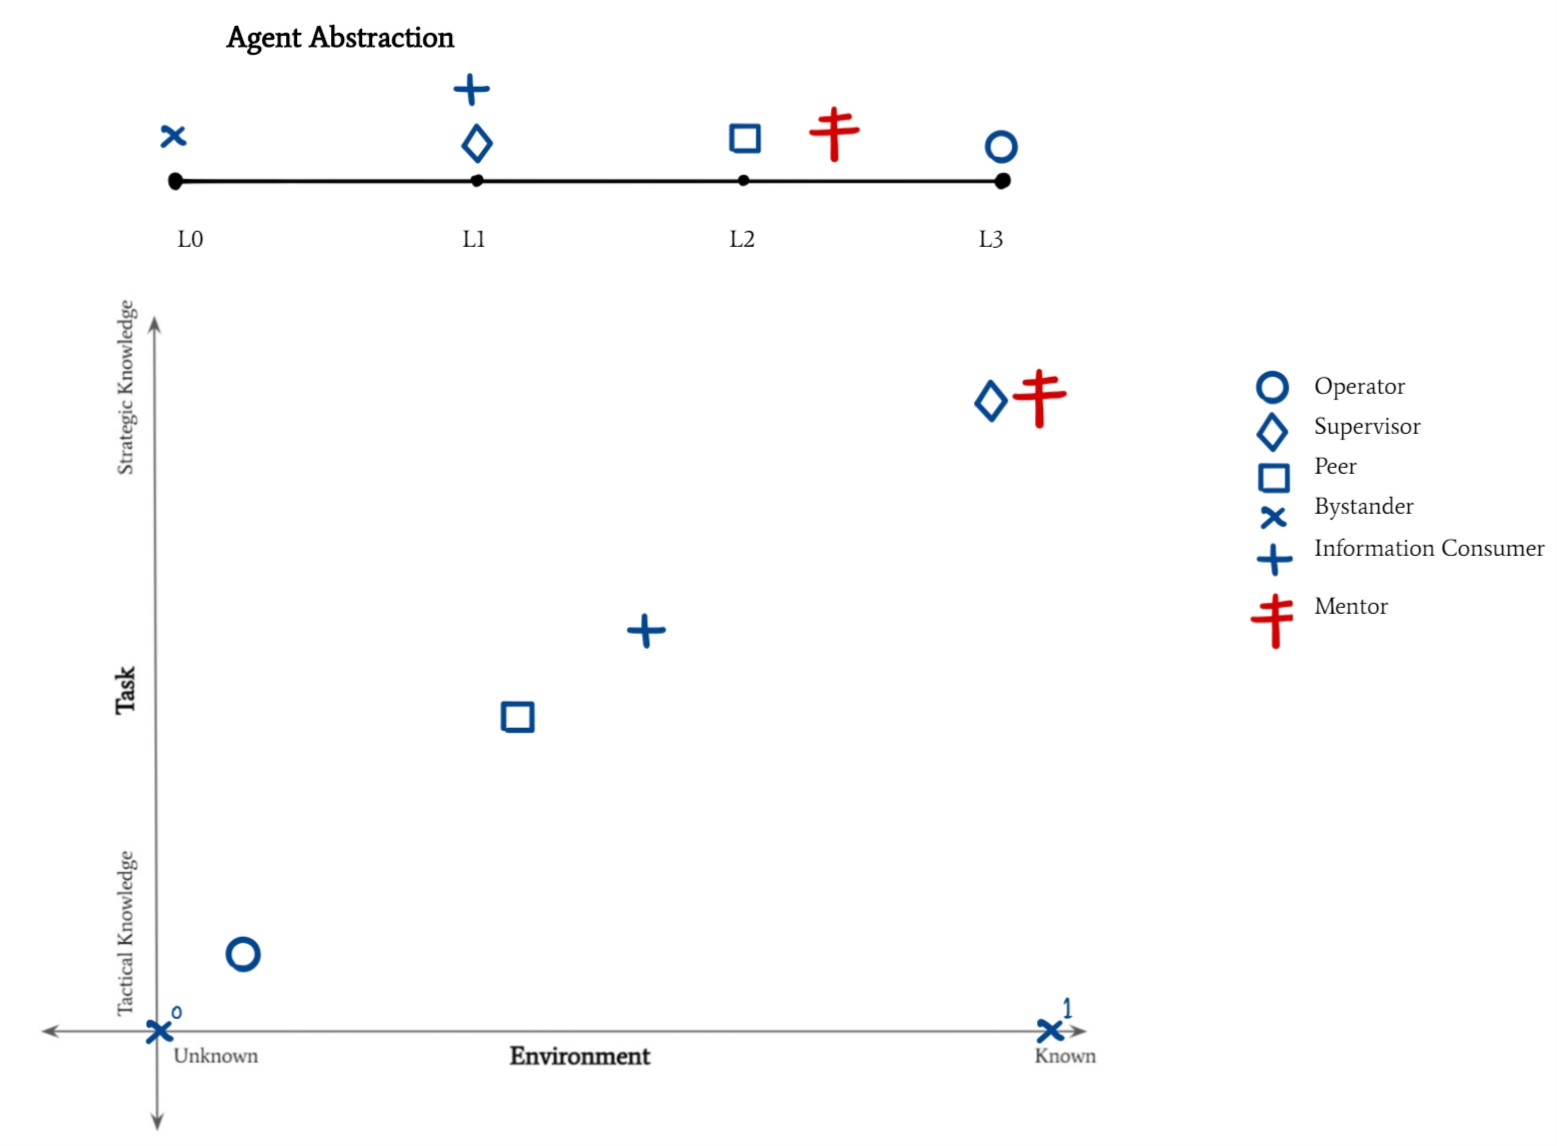
\includegraphics[width=\columnwidth]{role-dims.jpg}
   \caption{Roles sorted on the dimensions of a priori knowledge of: (a) Agent abstraction, (b) Task and (c) Environment}
    \label{fig:role-dims}
\end{figure}

Figure \ref{fig:role-dims} summarizes this distinction between roles based on the dimensions of a priori SA in task, environment and level of abstraction of the other agent.
}

\section{A Reformed Upper Ontology for Analyzing HRI Problems}
\label{sec:upper-ontology}

Following from the analysis in the previous section, here we propose our reformed upper ontology over the surveyed taxonomies.
We situate the taxonomies within this new structure and compound there insights over similar topics to break-down complex aspects systematically.

\subsection{SYSTEM CONTEXT}
Variables that fall under the context category function as independent variables for a given situation taken as inputs to the HRI problem. 

% \begin{table}[htb]
% \centering
% {\scriptsize 
% \begin{tabular}{ |c|c|c|c|c| } 
%  \hline
%  Factor & Modeling & Observability & Type & Constraints\\ 
%  Task & \cite{cao1997cooperative, Dudek2002updated} & \cite{cao1997cooperative} & \cite{Phillips2015,Beer2017} & \cite{Beer2014toward, Goodrich2007, Yanco2004updated}\\ 
%  Environment & Novel & Novel & \cite{Dautenhahn, Yanco2004updated} & N/A\\ 
%  Team & Novel & Novel & \cite{cao1997cooperative, Dudek2002updated, Yanco2004updated} & \cite{Goodrich2007, Yanco2004updated} \\ 
%  \hline
% \end{tabular}
% }
% \caption{Motivating Taxonomies for Contextual Factors}
% \end{table}

\begin{enumerate}

\item \textbf{TYPE.}
    Each major class in the contextual ontology is ascribed a stereotypical set of properties which help encapsulate the expected complexities the agents face from their task, environment or team-formation.
\begin{enumerate}
    \item \textit{Task.}
    Builds on task type taxonomies introduced in \cite{Phillips2015, Beer2017}.
        \begin{enumerate}
            \item \textit{Requirement Type.} \cite{Phillips2015} -
            \begin{enumerate*}
                \item \textit{Physical},
                \item \textit{Cognitive}, and
                \item \textit{Social}.
            \end{enumerate*}
            \item \textit{Task Focus.} \cite{Beer2014toward} -
            We add a new entry to this list (*) to incorporate the training and learning phase of interactions as seen in domestic and other social domains.
            \begin{enumerate*}
                \item transit,
                \item area coverage,
                \item resource management,
                \item target search,
                \item construction,
                \item assistance, and
                \item *learning of task \cite{fitzgerald2016situated, fitzgerald2018human, Cakmak2010} or environment \cite{kruijff2006clarification, topp2006topological, topp2010detecting, peltason2009mixed}.
            \end{enumerate*}
        \end{enumerate}
    \item \textit{Environment.}
    Focuses on capturing environmental macro-complexities by the way of following:
        \begin{enumerate}
            \item \textit{Expected Dynamics.} \cite{Dautenhahn, Burke2004} -
            Motivated by discussion of contexts in \cite{Burke2004}and ``contact with humans'' dimension in \cite{Dautenhahn}.
            \begin{enumerate}
                \item LOW - \cite{yamada1997human}
                \item FREQUENT - \cite{Casper2003}
                \item HIGH - \cite{Thrun1999Minerva, Burgard1999Mesuem, pacchierotti2006design}.
            \end{enumerate}
            {
            \color{blue}
            \item \textit{Hazard-level.}
            A new categorization motivated by different application contexts defined in \cite{Burke2004}, with conditions harmful for human survival versus other everyday human-inhabited environments.
            A binary property with assignments: \textit{TRUE} and \textit{FALSE}.
            }
        \end{enumerate}
    \item \textit{Team.}
        \begin{enumerate}
            \item \textit{Composition.} \cite{Dudek2002updated, cao1997cooperative} - 
            \begin{enumerate}
                \item \textit{HOMOGENEOUS} \cite{kitano1997robocup}
                \item \textit{HETEROGENEOUS} \cite{Karma2015, fitzgerald2018human}
            \end{enumerate}
            This composition is applied to the sub-team of interactants being scrutinized under this taxonomy.
            \item \textit{Cardinality.}
            Motivated by survey of operational contexts and size dimension in \cite{Dudek2002updated, cao1997cooperative}.
            \begin{enumerate*}
                \item \textit{One-to-One} \cite{fitzgerald2018human},
                \item \textit{One-to-Many} \cite{Thrun1999Minerva, Burgard1999Mesuem},
                \item \textit{Many-to-One}, \cite{li2013communication} and
                \item \textit{Many-to-Many}.
            \end{enumerate*}
        \end{enumerate}
\end{enumerate}
\item \textbf{MODELING.}
The modeling aspect of task, environment, and team context describes what information about each of the three is available to the team a priori, i.e. before task execution.
This helps in anticipating the information gap during execution and guides sensing, communication, and inference actions online.\footnote{It should be noted that every team member does not need all state information in most cases, and as will be discussed in the section regarding local dynamics.}

\begin{enumerate}
    {
    \color{blue}
    \item \textit{Task.}
    Motivated by our analysis of operational contexts with varying understanding of task models.
    Can take the following values: \textit{FULL} \cite{Thrun1999Minerva} or \textit{PARTIAL} \cite{fitzgerald2018human, Casper2003}.
    \item \textit{Environment.}
    Motivated by \cite{Burke2004}, encapsulates whether the operational environment has a known underlying semantic structure or not, and whether the physical map is known a priori or not.
    \begin{enumerate}
        \item \textit{Structure}
        \begin{enumerate*}[(A)]
            \item \textit{Structured}, e.g. an industrial workplace,
            \item \textit{Partially structured}, e.g. an office setting and
            \item \textit{Unstructured}, e.g. domestic setting or USAR scenario.
        \end{enumerate*}
        \item \textit{Mapping}
        \begin{enumerate*}[(A)]
            \item \textit{Mapped} in which a full map of the environment is available.
            \item \textit{Partially Mapped} in which some information is available, but the current state might have changed requiring adaptability, and finally
            \item \textit{Unmapped} in which no information about the environment is available a priori.
        \end{enumerate*}
    \end{enumerate}
    }
    \item \textit{Team.} \cite{stone2000multiagent, cao1997cooperative, chen2018situation} -
    \begin{enumerate}
        \item Shared-knowledge structures \cite{stone2000multiagent}
        \item Decision functions \cite{stone2000multiagent, chen2018situation}
        \item Action repertoire \cite{cao1997cooperative, stone2000multiagent, chen2018situation}
        \item Capabilities - Sensors, and effectors \cite{cao1997cooperative, stone2000multiagent}
    \end{enumerate}
\end{enumerate}

{
\color{blue}
\item \textbf{OBSERVABILITY.}
As compared to task modeling which demonstrates where a priori gaps lie in knowledge and what information would be required during task execution, observability considers what information is possible to sense, communicate, or infer during task execution and consequently which gaps are possible to close.

\begin{enumerate}
    \item \textit{Task.}
    \textit{PARTIAL} and \textit{FULL} observability of task refer to whether unknown aspects of a task specification, such as constraints or objectives, can be observed online during task execution. This categorization is motivated by the military building breach and interactive learners/museum docents operational contexts in which task specifications are not fully known a priori and must be learned online. \cite{cao1997cooperative} reviews work in a 'learning' dimension which discusses reinforcement learning techniques for ascertaining unknown aspects of task, but formal dimensions are not provided.
    %Partial and full task observability describe which unknown aspects of a task specification can be observed online during task execution. Unknown aspects of task specifications might include constraints or objectives of the task that might inform how teammates approach a task and share information. In some circumstances, certain unknown aspects of task specification may be unobservable in that they are too difficult to specify in a useful and intelligible way. For instance, \citet{gombolay2016apprenticeship} explain that domain experts often have difficulty describing their decision-making processes, causing the codification of the relevant objectives in these problems to be difficult. Instead of aiming to observe objectives directly, they capture domain expert heuristics to guide task execution. In such cases, proxies such as policies can be used, but the direct objective function is effectively unobservable. 
    
    \item \textit{Environment.}
    Partial and full observability of the environment describe whether some or all states relevant to task execution in the environment can be observed by agents performing a task.
    \begin{enumerate}
        \item Partial \cite{hadfield2016cooperative}
        \item Full \cite{nikolaidis2017game}
    \end{enumerate}
    
    \item \textit{Team.}
    When considering observation in terms of the team and its individual members, we consider both observability of teammates and the dual of this concept, defined as the observation ability of the team. Both of these categorizations are motivated by the operational contexts in which relevant factors driving decision-making of team members are not fully known and in which team members do not have full observation capabilities of relevant contextual factors.
    \begin{enumerate}
        \item Observability\\
            Observability of teammates parallels observability of task and environment and can be categorized as either \textit{PARTIAL} or \textit{FULL} observability. 
        \item Observation Ability\\
            As with observability, observation ability of the team can either be \textit{PARTIAL} or \textit{FULL}, meaning the team can either observe all possibly accessible state information relevant to task execution in the environment or a subset of the available information given its sensing and reasoning capabilities.
    \end{enumerate}
    
    %Observability of teammates parallels observability of task and environment and can be categorized as either PARTIAL or FULL observability. Partial observability of teammates arises when there are latent states impacting a teammate's actions that cannot be known directly \cite{unhelkar2018learning}. 
    
    %As with observability, observation ability of the team can either be partial or full, meaning the team can either observe all possibly accessible state information relevant to task execution in the environment or a subset of the available information given its sensing and reasoning capabilities. It should be noted that both observability of the team and observation ability of the team can be defined for interactions between one to two teammates or over the whole team.
\end{enumerate}
}

\item \textbf{CONSTRAINTS.}
This trait consists of latent aspects of a class as well as effect of type-complexity on other lateral factors which affect interaction.
\begin{enumerate}
    \item \textit{Task.}
        \begin{enumerate}
            \item \textit{Criticality.}\footnote{Our ontology addresses this aspect at the macro-level, but note that detailed frameworks exist \cite{lin2008autonomous} for a finer context-sensitive assessment.} \cite{Beer2014toward, Yanco2004updated} -
            We divide this aspect into two dimensions: criticality towards mission success, and criticality towards human-safety.
            Under the current state of robotic abilities and intelligence, the human-safety axis should have precedence over the task-critical axis when deciding for trade-offs between multiple action options.
            We suggest the following breakdown:
            \begin{enumerate}
                \item \textit{LOW} - Neither mission-critical, nor affects human-safety.
                \item \textit{MEDIUM} - Mission-critical, does not affect human-safety.
                \item \textit{HIGH} - Critical to human-safety.
                \item \textit{SEVERE} - Mission as well as safety critical.
            \end{enumerate}
        \end{enumerate}
    \item \textit{Team.}
        \begin{enumerate}
            \item \textit{Interaction Protocol.} \cite{Dautenhahn} -
            Motivated from ``requirement of social skills'' aspect in \cite{Dautenhahn} and our observations from study of operational contexts where either structured or social communication is strongly preferred.
            \begin{enumerate}
                \item \textit{Social protocols} \cite{Thrun1999Minerva, Burgard1999Mesuem, Cakmak2010, fitzgerald2018human, kidd2006sociable}
                \item \textit{Structured protocols} \cite{sheehan2004military, huckaby2012taxonomic}.
                % Could be in a social or structured setting but the modality for inputting information and commands, and eliciting information is constrained so the task description or questions are structured.
                % However the field is still open for using unmodeled gestures, expressions and social cues.
                % Example, military, naval, air traffic-control, etc.
            \end{enumerate}
            \item \textit{Spatial Relationship.} \cite{Yanco2004updated, Goodrich2007, Fong2003} - 
            We assign two high-level values to this aspect, i.e. \textit{PROXIMAL} or \textit{REMOTE}.\footnote{Although we do not include social proxemics \cite{hall1963system} explicitly in our taxonomy, it is worth mentioning that while looking at social interactions this axis should also be considered.}
        \end{enumerate}
\end{enumerate}
\end{enumerate}

\subsection{LOCAL DYNAMICS}
As compared to context variables, local dynamics variables are factors regarding team-work and task-work structure \cite{Mathieu2000TheIO} which impact how effectively a team can execute a task given the constraints imposed by contextual factors.


\begin{enumerate}
    \item Task
    
    % \begin{table}[htb]
    % \centering
    % {\small
    % \begin{tabular}{ |c|c|c|c| } 
    % \hline
    % Factor & Planning & Task Dependencies & Goal Dependencies\\ 
    % Task & \cite{GerkeyMataric2004, Korsah2013} & \cite{Beer2014toward, JiangArkin2015, Phillips2015, Phillips2012, Korsah2013, GerkeyMataric2004} & \cite{JiangArkin2015, Beer2017}\\ 
    % \hline
    % \end{tabular}}
    % \caption{Motivating Taxonomies for Task-Related Dynamics Factors}
    % \end{table}
    
        \begin{enumerate}
            \item \textit{Planning.} \cite{Korsah2013, GerkeyMataric2004} -
            We reformulate the instantaneous (IA) and time-extended (TA) task-assignment categorizations proposed in \citet{GerkeyMataric2004, Korsah2013} as more generic online and offline task planning, respectively.
            
            \item \textit{Task Dependencies.} 

            Our definition of task interdependence is based on review of taxonomies classifying properties of task allocation and interdependence \cite{Korsah2013, GerkeyMataric2004, Phillips2015, Phillips2012}. We adopt the four iTax classifications as defined by \citet{Korsah2013}:
            
            \begin{enumerate}
                \item No Dependencies
                \item In-Schedule Dependencies
                \item Cross-Schedule Dependencies
                \item Complex Dependencies
            \end{enumerate}
            
            
            While \cite{Korsah2013} focuses primarily on algorithmic solutions to task decomposition and task allocation, the categories proposed also apply to interaction. The task allocation within the team and the interdependence between the tasks that teammates are assigned in pursuit of the joint goal drives what information needs to be shared between them. We adopt the four primary categories proposed in \cite{Korsah2013} for task schedule dependencies as they relate to task decompositions: No Dependence, In-Schedule Dependencies, Cross-Schedule Dependencies, and Complex Dependencies. 
            
            Further, at a second level and borrowing from [Mataric and Gerkey], the axes of task type (single-robot or multi-robot), allocation type (instantaneous assignment or time-extended assignment), and robot type (single-task or multi-task) are defined. We adopt these categorizations, noting that although this classification deals with multi-robot task allocation in particular, in heterogeneous teams operating with both humans and autonomous agents in complex environments, humans and autonomous agents are considered interchangeably. 
            
            In this taxonomy, both task decomposition and task allocation to team members performing the tasks are of import. 
            \item \textit{Goal Dependencies.}
            For classification of goal dependencies, we use the categorizations proposed by \citet{Beer2014toward} to distinguish three general goals that contribute to achievement of any task: \textit{SENSE}, \textit{PLAN}, and \textit{ACT}.
            
            Each of these three goals can be filled by two or more teammates, classified as a \textit{JOINT} approach, or by a single teammate, classified  as \textit{INDIVIDUAL}. These categorizations are adopted from \citet{JiangArkin2015}.
            
            Given a task decomposition and allocation to team members, one or more teammates may share in the sensing, planning, or acting aspects of working towards a shared task. We further classify each of the three goals as either joint in which two or more teammates work together, or individual in which a single teammate works towards the specified goal. 
        \end{enumerate}
    \item Team
    
    % \begin{table}[htb]
    % \centering
    % {\small
    % \begin{tabular}{ |c|c|c|c| } 
    % \hline
    % Factor & Roles & Expertise Hierarchy & Communication\\ 
    % Team & \cite{Goodrich2007} & \cite{cao1997cooperative,Dudek2002updated, Yanco2004updated} & \cite{cao1997cooperative,stone2000multiagent, Dudek2002updated}\\ 
    % \hline
    % \end{tabular}}
    % \caption{Motivating Taxonomies for Team-Related Dynamics Factors}
    % \end{table}
    
        \begin{enumerate}
            \item \textit{Roles.}
            {
            \color{blue}
            Following from our discussion in the last section \ref{sec:analysis} we break-down the concept of roles along the dimensions of:
            \begin{enumerate}
                \item A priori Task Knowledge,
                \item A priori Environment Knowledge,
                \item A priori Level of familiarity with other agents
            \end{enumerate}
            Refer to sub-section \ref{subsec:stereotyping-roles} for a detailed breakdown of every role along these axes.
            }
           
            \item \textit{Expertise Hierarchy.} \cite{Dautenhahn} -
            As seen in \cite{Dautenhahn} roles are not always fixed properties.
            To capture this phenomenon in our taxonomy we divide expertise hierarchy into the following two dimensions:
            \begin{enumerate}
                \item \textit{Reconfigurability.}
                Motivated from spatial reconfigurability of teams in \cite{Dudek2002updated, cao1997cooperative}.
                Hierarchies can either remain \textit{FIXED} \cite{Casper2003, Thrun1999Minerva} or be \textit{FLUID} \cite{mortl2012role}.
                \item \textit{Decision-making Protocol.} \cite{Yanco2004updated, Dudek2002updated, cao1997cooperative} -
                The decision consensus protocol can be either: \textit{CENTRALIZED} or \textit{DISTRIBUTED}.
            \end{enumerate}
            \item \textit{Communication.}
            The communication model of the team as well as the capabilities of the individual interactants directly constrain information exchange \cite{stone2000multiagent, cao1997cooperative, Dudek2002updated}.
            \begin{enumerate}
                \item \textit{None or Environment-based} \cite{cao1997cooperative, stone2000multiagent} -
                There is no direct communication between the interactants, the agents are limited to observing the changes in environment or a connecting physical medium to infer other agents' actions and state.
                \item \textit{Sensing-based} \cite{cao1997cooperative} - 
                The interactants can only communicate by directly sensing the teammate and observing the actions and state.
                \item \textit{Direct-Partial} \cite{cao1997cooperative, Dudek2002updated} -
                The interactants have a communication channel but are limited by range-of-communication.
                \item \textit{Direct-Full} \cite{cao1997cooperative,stone2000multiagent, Dudek2002updated} -
                Interactants can communicate with any teammate, anywhere within the known environment.
            \end{enumerate}
        \end{enumerate}
\end{enumerate}

\subsection{EFFECTS}
Effects are resultant factors driven by the operational context of a team and the chosen dynamics for achieving the joint goal.
Given the  context, and task and team dynamics under our taxonomy, the level of autonomy of each teammate and the level of information abstraction for communicating with them should be set accordingly. 
\begin{enumerate}
    \item \textit{Level of Autonomy.}
    We adopt the levels of automation defined by \citeauthor{Beer2014toward} \cite{Beer2014toward}. In \cite{Beer2014toward}, levels of automation are determined in three modes of operation: sense, plan, and act. Ten levels are delineated, assigning the sense, plan, and act modes of operation to the human, the robot, or both the human and the robot together. In this upper ontology, and as we move into a world in which autonomous agents have capabilities that extend beyond traditional robot roles, we expand the designation of human and robot roles in this classification of levels of automation to include any two teammates or sub-teams interacting within the larger team.
    
    Decision of level of autonomy is based on what role a given teammate has assumed and in what context. For example, an operator executing a task in a fully-observable and fully-modeled context might operate at a higher level of automation than an operator executing the same task with a partial model or partial observability. In the latter case, the operator might rely more heavily on teammates to gather and communicate the necessary information and provide instruction. 
    
    %Level of autonomy is closely related to both the task dynamics and the team dynamics in that task dynamics drive required interaction and dependence between teammates or sub-teams performing different tasks towards the common goal and team dynamics influence the roles different teammates or sub-teams play and the dependence between those roles. 
    
    %Also important to consider regarding team and task dynamics is the level of autonomy assumed by each teammate or sub-team in the heterogeneous team of humans and autonomous agents. 
    
    \item \textit{Level of Information Abstraction.}
    Grice's maxims \cite{grice1975logic} provide succinct guidelines for designing cooperative communication, and we wish to highlight two of those:
    \begin{itemize}
        \item \textbf{Maxim of Quantity} -- Be as informative as you can, and no more.
        \item \textbf{Maxim of Relation} -- Be relevant to the discussion.
    \end{itemize}
    
    These guidelines hint at a strong inter-dependence between information abstraction, ``issue'' being discussed and required situated awareness for better decision-making or discussion.
    Assuming agents interact rationally and discuss ``issues'' with the agents with the right expertise, then under our taxonomy we can use the \textit{team-roles} to provide us with the missing information.
    However, as has been hinted before in section \ref{sec:analysis}, an exact informational profile of a role would be needed to perform such assessments online.
    This grounded profile would include the expertise profile of each role, their expected level of knowledge in other vertical fields and their levels of familiarity with the agent's internal systems.
    We require these dimensions such that the information can be tailored to the nature of an interactant under the maxim of relation.
    % The \textit{a priori expertise} of various teammates can be used to identify the right interactant for discussing issues related to strategic plans, tactical moves, and environmental uncertainties.
    % Similarly, their \textit{a priori level of familiarity with an agent's model} can be used to provide agent's state and status information at the right abstraction level.
    
    Following the thread of situational awareness \cite{endsley1988design}, it is also important to know how much the interactants know about current state and status of each other.
    If the \textit{spatial relationship} is proximal then they have direct access to physical situatedness, however is the relationship is remote in nature then the interactants are charged with exchanging the cognitive as well as physical situatedness.
    By physical situatedness we mean level 1 aspects of \cite{chen2018situation} and by cognitive situatedness we mean the level 2 and level 3 aspects from the same paper.
    This helps in tailoring the communication as per the maxim of relation.
    
    Finally, the level of information abstraction also depends on the relevance of the state of either interactant to the other \cite{JiangArkin2015, Beer2014toward}.
    This relationship can be assessed along the dimensions of \textit{goal and task dependency}, outlined in our dynamics taxonomy.
    Our guidelines state that more the inter-dependency, finer the granularity of updates should be, conditioned on the fact that the updates should contribute to the constraints of dependency in a positive or negative way.
    Similarly, depending upon if the interactants have same or different goal the level of task abstraction should be adjusted such that the interactants share action or goal-level information, respectively.
    
\end{enumerate}

\section{Discussion}
\label{sec:discussion}

In this paper we surveyed taxonomies and frameworks from fields of human-robot interaction, algorithmic robotics systems and behavioral sciences to better understand their influence on each other and identify undocumented gaps to motivate future research.
We observed that the factors identified by surveyed taxonomies not only laterally interact with each other, but there is also a top-down pattern where higher-level factors affect the range of design choices over the factors below them.
As a result of this analysis, we propose an extensible taxonomy which breaks down an HRI system into three levels of depth: system \textit{context-model}, \textit{local dynamics-model} of the interaction, and resultant \textit{effects} on leaf factors driving human-robot interaction.
These levels are used to characterize three major system components: \textit{task}, \textit{environment} and \textit{team}.
We arranged the surveyed taxonomies within this framework, drawing on their insights on similar factors along different dimensions (figure \ref{fig:alt-upper-ontology}).

There are two main areas of focus in the undocumented gaps.
First, as we are moving towards ``true'' collaboration there is a demonstrated need in the surveyed literature for enhanced communication protocols, flexible role change, and adaptive communication for different kinds of human interactants.
This underscores the need for a situational-awareness-assessment framework which can be applied to all three system components of our taxonomy.
While, \cite{chen2018situation} grounds the principles of situational awareness as it applies to the mission specification of a system, there is still a space for conceptualization of a framework which extends this idea to environment and team configurations.
As per our survey, this would need to draw on the situational awareness principles \cite{endsley1988design}, and a more structured understanding of possible human and robot roles \cite{Scholtz2003, Goodrich2007}.
Second, most of these taxonomies are formulated by placing assumptions on the kinds of environment they address.
While this strengthens their insights for the specific interactions addressed, this also means that,
\begin{enumerate}[A)]
    \item These specific taxonomies do not include the environment as a major factor, and
    \item There is a dearth of taxonomies, in general, which characterize the specific challenges of different operational environments.
\end{enumerate}

We present an illustrative example by walking the reader through gaps in characterization of the outlined contexts in section \ref{sec:op-context} when only using the currently identified factors.
\begin{itemize}
    \item \textit{Lack of explicit environment modeling}, which results in omission of capturing environmental challenges important to design decisions.
    \begin{itemize}
        \item This obscures the risk to the human operator from the environment in scenarios \ref{subsec:usar} and \ref{subsec:mbb}, which directly affects the recommended autonomy level for the robot's end of perception task such that the operator is not cognitively overloaded.
        \item Knowledge of semantic and physical mapping drastically affects the information exchange patterns in the IL scenario in \ref{subsec:il-and-md} versus \ref{subsec:mbb}.
        While the former requires task or plan information to learn better, the latter also requires information exchange about the physical aspects of the context.
        \item Even within the niche domain of IL in \ref{subsec:il-and-md}, some demonstrations are given in physically proximate configuration while some are remote.
        Unless explicitly modelled this information just by itself does not tell us if the demonstrator already has a mental-model of the environment, or is seeing it for the first time.
        Factors like this directly factor in learning ability of a system as well as its applicability in different domains.
    \end{itemize}
    \item \textit{Lack of observability modeling} during execution, which obscures the distinction between what is available and what needs to be shared. For example, in \ref{subsec:mbb}, the teams are distributed over a large area and have limited observability of the space as well as their teammates.
    This entails that during execution the members need to relate information about spaces, events and their own state to others.
    An important considerations is how much should be shared in order to avoid overloading the other interactant.
\end{itemize}

While our taxonomy takes a first step towards defining such challenges by identifying dimensions proposed from a different lens but applicable to system context, like \textit{expected dynamics} and \textit{team reconfigurability}, there is still a requirement for a deeper characterization.
Such an investigation can help in analyzing operational contexts for HRI in a standardized manner such that the insights from one taxonomy can be generalized or conditioned from one context to another.

\subsection{OLD}

One of our goals is to define an upper ontology over the taxonomies mentioned in the previous section, as a na\" ive tool which can help a reader in describing and analyzing the interactions in their mixed teams.
Drawing from our insights in section \ref{sec:op-context}, we establish the ``Task, Environment and Team Context'' as the main differentiating dimensions for operational contexts.
The above make the starting set of independent variables in our analysis.
This is also consistent with the taxonomies identified in section \ref{sec:before-hri} and the context-first taxonomies in section \ref{subsec:context-taxonomies}.
In order to include the specifics arising from the particular use-case engaged in interaction, we introduce another tier for ``Team and Task Dynamics''.
This tier is influenced by the teamwork and task-work distinction imposed by cognitive scientists to analyze performance of a team \cite{Mathieu2000TheIO}.

If we try to cluster the factors mentioned in section \ref{sec:survey}, we find multiple mentions of task type (albeit at different levels of abstractions), task criticality, spatial configurations, and human roles.
Since we are trying to characterize and differentiate between high-level operational contexts, we include the task type definition given in \cite{Phillips2015}, i.e. cognitive versus physical.
Task criticality is a function of the application context of a human-robot collective.
Spatial configuration and the human role are a fixed artifact of the specific team hierarchy that the interactants belong to.
To be consistent with our definitions of the higher-level categories, we include task type and criticality as a part of task context, and include spatial configuration and roles as a part of team dynamics.
Our next quest is to look at the specific use-cases more deeply and identify a range of configurations for these factors which help in differentiating between the use-cases.

\subsection{Context}
\subsubsection{Environment}

\paragraph{Mapping}
Based on the taxonomies on communication modality and the short review of operation contexts, the environmental factor is characterized over two dimensions: mapping - a simple axis of known versus unknown, and affordance over land, sky and water which affects the composition of the robot agents used.

\paragraph{Traversability}

%\paragraph{Observability (LMS)}
%Another environment-based driver of interaction in observability of the environment. While mapping affects what information about the environment is needed within the team, observability impacts what information is actually available to be shared. We define two subcategories for classification: fully-observable and partially-observable. We note that full-observability and partial-observability should be defined only over factors influencing decision-making within the team. 


\subsubsection{Task}
\paragraph{Risk (LMS to Modify)}
Task criticality is a unique aspect that warrants a deeper look.
Importance of this aspect comes into play when deciding the correct levels of autonomy for a system.
One of the foremost questions that \citeauthor{Beer2014toward} ask about the task in \cite{Beer2014toward} is to determine what is the criticality and accountability of a task?
The context review for USAR and museum docents highlighted the fact how safety of the agent (for operator) and safety of the bystanders during navigation are one of the main concerns during execution.
Therefore, we file this under task-context as 'risk factor' and break it down into two components: risk towards human and the environment, and risk for the agent. 

LMS - 

\paragraph{Type}
We saw task interdependence and type of task requirement as two important axes for human-animal collaboration.
However, task interdependence arises out of the specific dynamics and capabilities of the team, therefore we file this under the dynamics category.
And to ground our ontology in the applications of today we select type of task requirement as the other component of task context.

\subsubsection{Team}

\paragraph{Cardinality - ?}
Perhaps the dimensions here are single agent versus multi-agent?

Similarly for team context we include the cardinality of the interactants engaging in the current interaction.
This dimension is inspired by our use-case studies and exists so that we can differentiate between the forms of communication which support multiple agents versus one.

\paragraph{Composition - ?}
Dimensions of heterogeneous or homogeneous?

\paragraph{Observation Ability - ?}
Does the team have the ability to fully observe available state information? A counterpart to observability in the enviornment. Possible dimensions of "full observation ability" and "partial observation ability".

\subsection{Task and Team Dynamics}

Context refers to the larger operational context of a mission/task, however the specific instantiation of this task gives rise to local dynamics which are the subject of our discussion next.
For our task and team dynamics, we have three sub-components: task interdependence, spatial configurations and roles.
Task interdependence borrows from the concise scale defined in \cite{Phillips2015}: pooled, sequential and reciprocal.

For spatial configurations we use the simple differentiator of proximal versus remote.
Proximal denotes configurations where interactants are near each other up-to a visible distance, remote denotes all configurations where the interactants can not observe each other directly \cite{Cha2018, Kolling2016}.
Finally for human roles we adopt 6 of the 7 roles outlined in section \ref{subsec:social-taxonomies}, omitting the mechanic.
The discussion above fulfills the first part of this paper's contribution, i.e. characterizing a collaborative problem.

This ontology is presented in figure \ref{fig:full-upper-ontology}.

\subsubsection{Task}
\paragraph{Task and Schedule Dependencies}

\paragraph{Online/Offline - Rename this}
\paragraph{Single-Agent Task/Multi-Agent Task}
%\subsubsection{Task Interdependence - LMS - IN PROGRESS}
%Throughout our survey we highlighted the different interpretations HRI and behavior science community has placed on the concept of interdependence \cite{Korsah2013, GerkeyMataric2004, Jiang2015mixed, Beer2014toward, Naderi2001}. We conceptualize task interdependence as the fundamental effect of task workflow and goal-overlap between the interactants. 
%We present an analysis of this concept over the following primary dimensions as identified through this survey:
%\begin{itemize}
    %\item \textbf{Task workflow or scheduling constraints.} Naderi et al. pooled, reciprocal, sequential and Korsah's dependencies.
    %\item \textbf{Goal-overlap.} Jiang and Arkin's goal-overlap, Beer et al.'s LORA framework
%\end{itemize}
%Our definition of task interdependence borrows from the taxonomy proposed in [cite Korsah] which also builds on the work of [cite Mataric and Gerkey]. While these taxonomies focus primarily on algorithmic solutions to task decomposition and task allocation, the categories proposed also apply to interaction. The task allocation within the team and the interdependence between the tasks that teammates are assigned to do in pursuit of the joint goal drives what information needs to be shared between them. In this taxonomy, both task decomposition and task allocation to team members performing the tasks are of import. [Korsah] defines four primary categories for task schedule dependencies as they relate to task decompositions: No Dependence, In-Schedule Dependencies, Cross-Schedule Dependencies, and Complex Dependencies. Further, at a second level and borrowing from [Mataric and Gerkey], the axes of task type (single-robot or multi-robot), allocation type (instantaneous assignment or time-extended assignment), and robot type (single-task or multi-task) are defined. We adopt these categorizations, noting that although this classification deals with multi-robot task allocation in particular, in heterogeneous teams operating with both humans and autonomous agents in complex environments, humans and autonomous agents are considered interchangeably. 

\paragraph{Team}
\subsubsection{Roles}


\subsubsection{Levels of Autonomy - LMS}
Also important to consider regarding team and task dynamics is the level of autonomy assumed by each teammate or sub-team in the heterogeneous team of humans and autonomous agents. Level of autonomy is closely related to both the task dynamics and the team dynamics in that task dynamics drive required interaction and dependence between teammates or sub-teams performing different tasks towards the common goal and team dynamics influence the roles different teammates or sub-teams play and the dependence between those roles. We adopt the levels of automation defined by [cite Beer]. In [cite Beer], levels of automation are determined in three modes of operation: sense, plan, and act. Ten levels are delineated, assigning the sense, plan, and act modes of operation to the human, the robot, or both the human and the robot together. In this upper ontology, and as we move into a world in which autonomous agents have capabilities that extend beyond traditional robot roles, we expand the designation of human and robot roles in this classification of levels of automation to include any two teammates or sub-teams interacting within the larger team. 

Clearly a close connection to the 'roles' sub-category in the upper ontology exists. For instance, the 'Supervisory Control' level designated by [Beer] involves the robot sensing, planing, and acting, and a human monitoring and having override capability to set a new goal or plan. In future teams, an operator might take the play the role of the robot defined in the 'supervisory control' level, and a supervisor in our framework would act as the supervisor within the framework in [Beer]. The distinction lies in the fact that either a human or an autonomous agent can play any role within our framework. 
[TODO: Write in how this drives communication/interaction]

\begin{figure*}[h!]
    \centering
    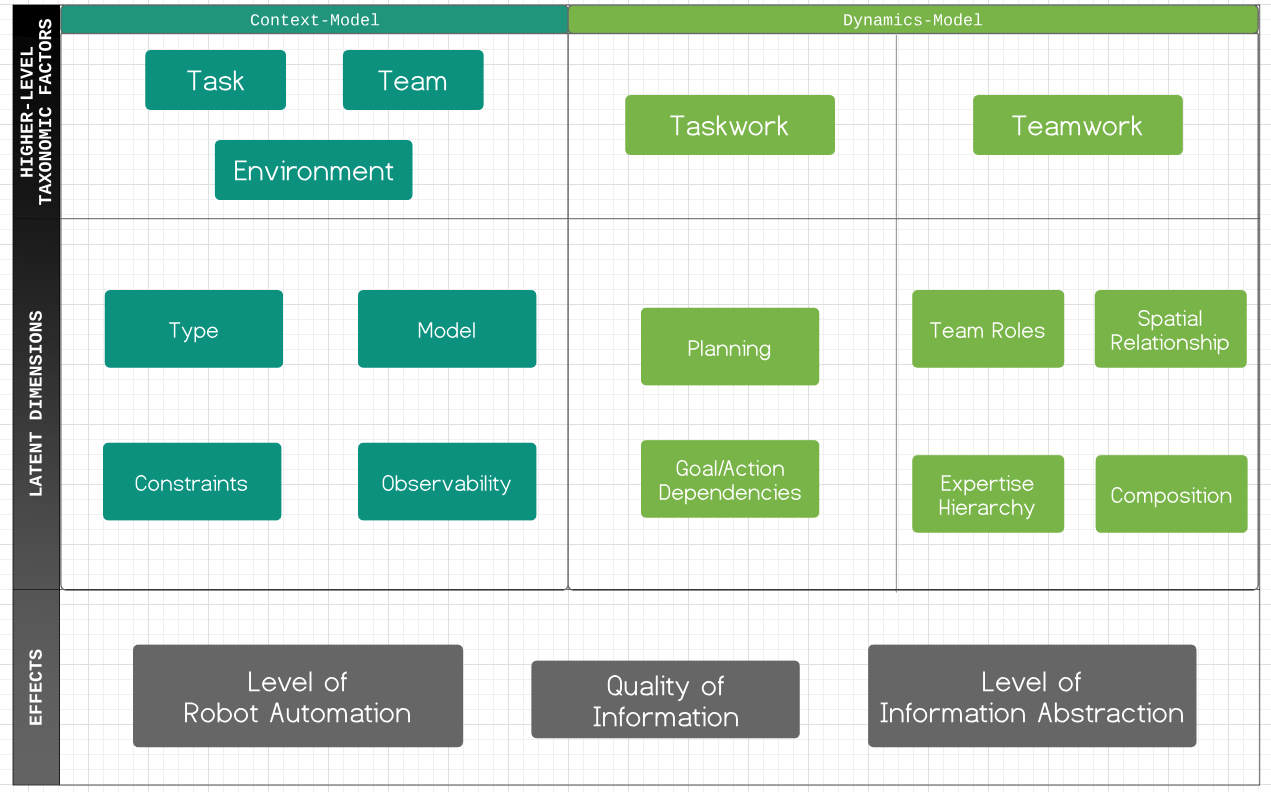
\includegraphics[width=0.85\textwidth]{alt-ontology.png}
    \caption{Alternative Visualization for the Upper Ontology.}
    \label{fig:alt-upper-ontology}
\end{figure*}

\subsection{OLD - Informational Interaction}

Before answering the above question, lets briefly ruminate on the concept of interactions as a way of communicating knowledge, rather than specific contexts of control, command and awareness.
Communication is a general umbrella that covers any kind of information exchange.
Grice's maxims \cite{grice1975logic} are guidelines for shaping communications, via an insight into the interaction between logic and conversation:
\begin{quote}
    \begin{itemize}
        \item \textbf{Maxim of Quantity} -- Be as informative as you can, and no more.
        \item \textbf{Maxim of Quality} -- Do not give untruthful information or information not supported by evidence.
        \item \textbf{Maxim of Relation} -- Be relevant to the discussion.
        \item \textbf{Maxim of Manner} -- To be clear, brief and orderly in what is communicated
    \end{itemize}
\end{quote}

The maxim of manner directly maps to our notion of communication modalities, i.e. what is the best way to communicate the required information?
Maxim of quality for an autonomous agent is supported by the law of probabilities, if there is not sensory evidence for a claim or a technological reason for an assertion then it won't be made.
For the scope of this paper, let's make an assumption that the human teammates are also bound by this law due to a mutual interest in achieving the goal quickly and correctly.

The maxim of quantity relates back to the quote \ref{quote:abstraction} we made in section \ref{subsec:interactive-learner}.
Each human cast in one of the prototypical roles (section \ref{subsec:social-taxonomies}) has knowledge of a different abstraction of the robot/autonomous agent.
By modeling this aspect we can provide guidelines for adhering to the maxim of quality.
The maxim of relation maps with our category of dynamics between the two interactants.
In order to be relevant to the expected discussion, we need to understand where the human and agent are situated in the task landscape as well as the environmental landscape.
This connects back to the combined task and environment SAT model defined in \cite{chen2014situation}.
However, this model is based on the information to be provided at execution, we still need to connect this with a human factor which is that by knowing about the task or environment awareness how are they helped in leveraging their expertise?
This connect us back to the definition \ref{def:cooperation} of cooperation, and the concept of situational awareness we explored in the last section.
While the definition provided for situational awareness in previous section works for analyzing a lone system's SA, \cite{Endsley1995} refines this model to aide the study of joint SA via team-mate interaction.
\citeauthor{Endsley1995} here keeps the same model for dynamic decision making with the levels of SA, however he also adds a delineation between ``task/system factors'' and ``individual factors'' which together affect the overall SA level.
And this later category of individual factors is exactly what we are interested in examining.

\section{Discussion}
\label{sec:discussion}
In this paper, we proposed an upper ontology for characterizing interaction within heterogeneous teams in complex scenarios and introduced an a-priori-situation awareness framework to support it. This upper ontology builds on existing taxonomies by organizing existing categorizations from these works and defines new categorizations to classify problems involving task-, environment-, and team-related complexity.

The need to define a new upper ontology over existing taxonomies is demonstrated by the operational contexts discussed in section \ref{sec:op-context}.  In the museum docents and interactive learners context, while the environment is known, the task model is incomplete and there are numerous unmodeled interactants. In the USAR scenario, complexity arises from the lack of known structure and full mapping of the environment in addition the non-static assignment of roles to teammates. Finally in the military building breach scenario, teammates are operating in an unknown environment, the task is only partially modeled, and there exists a fluid team hierarchy. These operational contexts motivate the need for categories considering a priori modeling and online observability and also the need to classify level of automation and level of information as effects rather than static artifacts of a given context. 

The structure of the upper ontology developed in this work has highlighted some areas of interest for future work. First, for categorizations not delineated by existing taxonomies, more research is needed to examine the impact of these factors on interaction. These categories primarily include modeling and observability in the task, team, and environment contexts and a particular exploration of these ideas as they relate to large, heterogeneous teams. Additionally, further research is needed to explore the optimal relations between the context and dynamics variables and effects.  Developing a full mapping between given context and dynamics variables and the recommended levels of automation associated with each role and subsequent levels of information necessary for each role is an open area for further research. 

%In this paper, we proposed an upper ontology for characterizing interaction for heterogeneous teams working in novel and complex domains. One of the objectives of this work was to lay the groundwork from which the community can identify where gaps in the literature exist, but we see a few initial key areas for further research. First, solidifying the relation of the level of autonomy and level of information effects to the context and dynamics of a given scenario would be of benefit. While we provide general categorizations as a starting point, specific mappings of appropriate level of autonomy or level of information for each teammate in their given context is an important area for future work. Second, this and other gaps in the literature would be supported by additional observational studies to better characterize interaction in large heterogeneous teams. Finally, while the subject of much of the literature in this space has thus far dealt with interaction in teams of two to a few, interaction in larger heterogeneous swarms is a nascent and less-studied area. We therefore recommend using the factors outlined here to study interaction in larger teams.

%A review of the current state-of-the-art indicates that the areas of research fueling the collaboration of tomorrow are:
%\begin{itemize}
%    \item Adaptive automation \cite{parashar_goel_sheneman_christensen_2018}
%    \item Bi-directional communication
 %   \item More observational studies to better characterize interactions
 %   \item Better ways to communicate data over limited communication resources
 %   \item The paper also points out that for a truly companion-like behavior the ability to be shaped by learning than having closed functionality is essential for the robotic agent.
  %  \item next-point
%\end{itemize}{}

%\citeauthor{chen2018situation} \cite{chen2018situation} use the above proposed SAT model to design interfaces for remote control of one ground agent.
%Their results suggest that while SAT model helps in improving performances in some cases, it needs to be dynamic and bi-directional for adapting to the operator's individual differences.
%Additionally, they observe that conditioned on the a priori environmental awareness of the user the same level of information can produce different decisions.
%They present their results using a computer-based human-robot mediator called RoboLeader \cite{chen2010roboleader}, which provided next-goal options and SA information to the operator.
%They conducted an experiment where an agent was to be driven across the city but introduced weather-based disturbances into the map.
%They observed that having an advanced environmental knowledge via known maps, made the operators over-confident about their own reasoning about time-to-finish and over-ruled the (correct) detour suggestions offered by the mediator.
%This is in contrast to when the environment was unmapped and the operators trusted the decisions of the RoboLeader, and there was a higher agreement rate.


% \section*{Outline}

% \begin{enumerate}
%     \item Introduction \ref{sec:intro}
%     \item Op-context survey \ref{sec:op-context}
%     \begin{enumerate}
%         \item USAR
%         \item Interactive Learner and Museum Docent
%         \item Military Building Breach
%     \end{enumerate}
%     \item Taxonomy survey \ref{sec:survey}
%     \begin{enumerate}
%         \item Animal-human analogy \ref{subsec:human-animal}
%         \item Contextualizing interactions \ref{subsec:context-taxonomies}
%         \item social skills and constraints \ref{subsec:social-taxonomies}
%         \item information-centric taxonomies for function and types \ref{subsec:information}
%     \end{enumerate}
%     \item Taxonomic Characterization of Interactions \ref{sec:characterization}
%     \begin{enumerate}
%         \item Introduction - general major factors identified and outline of this section
%         \item Introduction of proposed terminology
%         \item Break-down of important concepts using above terminology
%         \item Placing everything in a Taxonomy
%     \end{enumerate}
%     \item Diagrams
%     \item Discussion and Conclusion \ref{sec:discussion}
% \end{enumerate}

\listoftodos

%\begin{table*}[h!]
%\centering
%\caption{Autonomy Modes \cite{Beer2014toward}}
%\label{table:autonomy-modes}
%\resizebox{\textwidth}{!}{%
%\begin{tabular}{lllll}
%\hline
%\textbf{LORA}                        & \textbf{Sense} & \textbf{Plan} & \textbf{Act} & \textbf{Description}                                                                                   \\ \hline
%Manual                               & H              & H             & H            & Human performs all action                                                                              \\
%Tele-operation                       & H/R            & H             & H/R          & Robot assists with action implementation, sensing and planning allocated to human                      \\
%Assisted Tele-operation              & H/R            & H             & H/R          & Human assists but the robot senses and chooses to intervene                                            \\
%Batch Processing                     & H/R            & H             & R            & Both monitor and sense the environment, human determines goals and plans                               \\
%Decision Support                     & H/R            & H/R           & R            & Both sense and generate a task plan, human chooses the task plan and commands robot                    \\
%Shared Control with Human Initiative & H/R            & H/R           & R            & Robot senses, develops plans and goals, and implements actions; human monitors and may intervene       \\
%Shared Control with Robot Initiative & H/R            & H/R           & R            & Robot performs all aspects; can prompt human for help during some difficulty                           \\
%Executive Control                    & R              & H/R           & R            & Human gives abstract, high-level goal, robot senses, plans and acts                                    \\
%Supervisory Control                  & H/R            & R             & R            & Robot senses, plans and acts; human monitors and has override capability and may set new goal and plan \\
%Full autonomy                        & R              & R             & R            & Robot performs all aspects autonomously                                                               
%\end{tabular}%
%}
%\end{table*}

%%%%%%%%%%%%%%%%%%%%%%%%%%%%%%%%%%%%%%%%%%%%%%%%%%%%%%%%%%%%%%%%%%%%%%%%%%%%%%%%

\printbibliography


\end{document}
